\section{Time Series}





\begin{frame}<1-2>{\currentname: City Score Definition}

    

    \begin{exampleblock}{\textsc{Score = }}
        \begin{flalign*}
            & {\only<2->{\color{red}} n\_killed\_week }*  {\only<2->{\color{green}} 1} + {\only<2->{\color{red}} n\_injured\_week} *  {\only<2->{\color{green}} 0.8} + {\only<2->{\color{red}} n\_arrested\_week} * {\only<2->{\color{green}} 0.5} \\
            &+ {\only<2->{\color{red}} n\_child\_week}  * {\only<2->{\color{green}} 1} + {\only<2->{\color{red}} n\_teen\_week }* {\only<2->{\color{green}} 0.8} + {\only<2->{\color{red}} n\_adult\_week} * {\only<2->{\color{green}} 0.5} \\
        \end{flalign*}
        \begin{flalign*}
            &n\_killed\_week = \text{number of killed people in a specific week} \\
            &n\_injured\_week = \text{number of injured people in a specific week} \\
            &n\_arrested\_week = \text{number of arrested people in a specific week} \\
            &n\_child\_week = \text{number of child participants in a specific week} \\
            &n\_teen\_week = \text{number of teen participants in a specific week} \\
            &n\_adult\_week = \text{number of adult participants in a specific week} \\
        \end{flalign*}

    \end{exampleblock}
\end{frame}

%%%%%%%%%%%%%%%%%%%%%%%%%%%%%%%%%%%%%%%%%%%%%%%%%%%%%%%%%%%%%%%%%%%%%%%%%%

\begin{frame}{\currentname: Time Series Overview}

    \begin{figure}
        \centering
        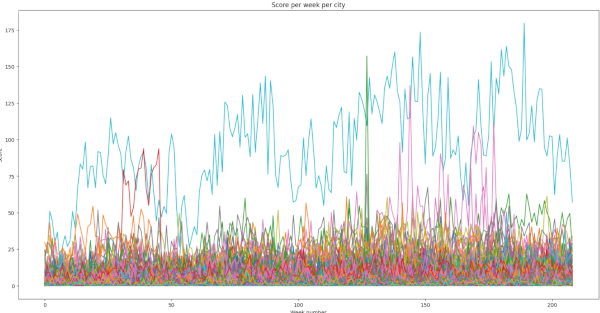
\includegraphics[width=.99\textwidth]{img/ts/a.png}
        \caption{Generated Time Series}
        \label{GTS}
    \end{figure}
    

\end{frame}


%%%%%%%%%%%%%%%%%%%%%%%%%%%%%%%%%%%%%%%%%%%%%%%%%%%%%%%%%%%%%%%%%%%%%%%%%


%TODO Make the various parts appear in order
\begin{frame}<1-3>{Clustering}
    \begin{minipage}{0.43\textwidth}
    
        
        \begin{exampleblock}{\textsc{Types of Clustering:}}
            \vspace{.8em}

            \begin{itemize}
                \item Standard Clustering
                \item Feature Clustering
            \end{itemize}
            \end{exampleblock}        
        
        
            \begin{exampleblock}<3->{\textsc{Algorithms utilized:}}        
                    
                \begin{itemize}
                
                    \item K-Means on Time series
                \end{itemize}
            \end{exampleblock}
        
    \end{minipage}
    \begin{minipage}{0.43\textwidth}
        

        \visible<2->{
        \begin{tabular}{|l|l|}
            \hline
            \textbf{Feature} & \textbf{Description} \\
            \hline
            'avg' & Mean (average) of the values. \\
            'std' & Standard deviation of the values. \\
            'var' & Variance of the values. \\
            'med' & Median of the values. \\
            '10p' & 10th percentile of the values. \\
            '25p' & 25th percentile of the values. \\
            '50p' & 50th percentile of the values. \\
            '75p' & 75th percentile of the values. \\
            '90p' & 90th percentile of the values. \\
            'iqr' & Interquartile range. \\
            'cov' & Coefficient of variation. \\
            'skw' & Skewness of the values. \\
            'kur' & Kurtosis of the values. \\
            \hline
        \end{tabular}
        }
        
    \end{minipage}
    
\end{frame}

%%%%%%%%%%%%%%%%%%%%%%%%%%%%%%%%%%%%%%%%%%%%%%%%%%%%%%%%%%%%%%%%%%%%%%%%%%

\begin{frame}{Silhouette Score}

    \begin{table}[htbp]
        \centering
        \begin{tabular}{|c|c|c|}
          \hline
          \textbf{n\_clusters} & \textbf{silhouette score original} & \textbf{silhouette score features}\\
          \hline
          2 & 0.812281 & 0.984422 \\
          3 & 0.781509 & 0.936071 \\
          4 & 0.625345 & 0.872255 \\
          5 & 0.458336 & 0.825605 \\
          6 & 0.458559 & 0.765932 \\
          7 & 0.461002 & 0.765437 \\
          8 & 0.424799 & 0.689629 \\
          9 & 0.413574 & 0.690026 \\
          \hline
        \end{tabular}
        \label{Silhouette Score for the different Scaling}
        \caption{Silhouette Score the Original Time Series and their Features}
      \end{table}      

\end{frame}
        


%%%%%%%%%%%%%%%%%%%%%%%%%%%%%%%%%%%%%%%%%%%%%%%%%%%%%%%%%%%%%%%%%%%%%%%%%%

\begin{frame}{Motifs and Anomaly Detection}

    \begin{figure}
        \centering
        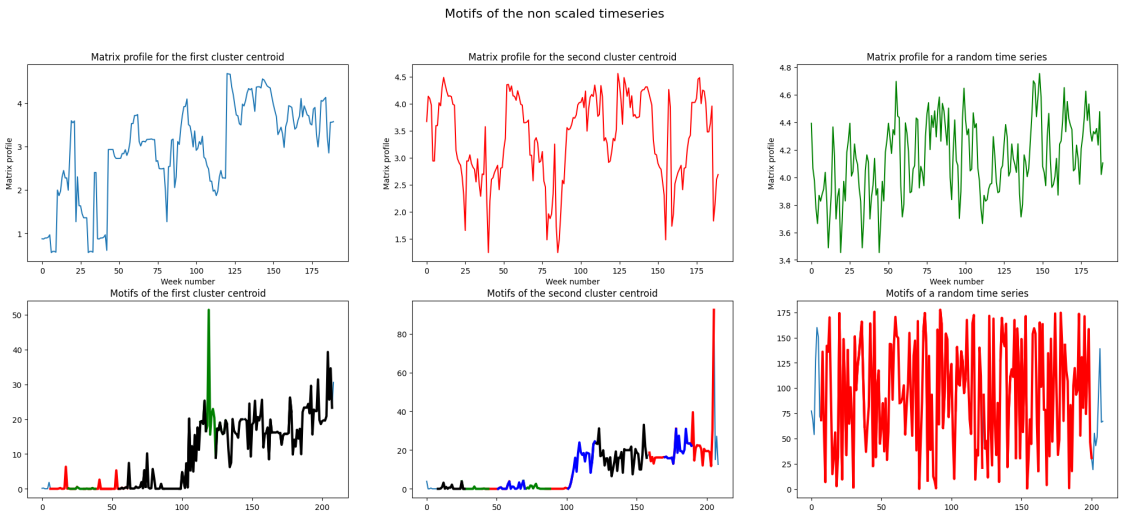
\includegraphics[width=.99\textwidth]{img/ts/Motifs.png}
      
        \label{MOT}
    \end{figure}
    
    
        
\end{frame}
        

%%%%%%%%%%%%%%%%%%%%%%%%%%%%%%%%%%%%%%%%%%%%%%%%%%%%%%%%%%%%%%%%%%%%%%%%%%

\begin{frame}{Motifs and Anomaly Detection 2}

    \begin{figure}
        \centering
        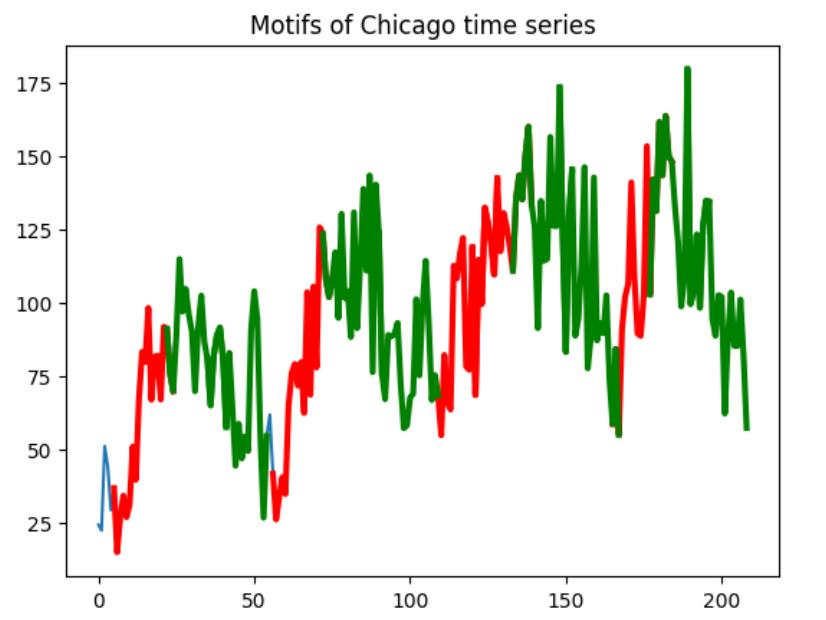
\includegraphics[width=.8\textwidth]{img/ts/ChicagoMotifs.png}
      
        \label{CHGMOT}
    \end{figure}
    
    
        
\end{frame}


%%%%%%%%%%%%%%%%%%%%%%%%%%%%%%%%%%%%%%%%%%%%%%%%%%%%%%%%%%%%%%%%%%%%%%%%%%


\begin{frame}{Motifs and Anomaly Detection 3}

    \begin{figure}
        \centering
        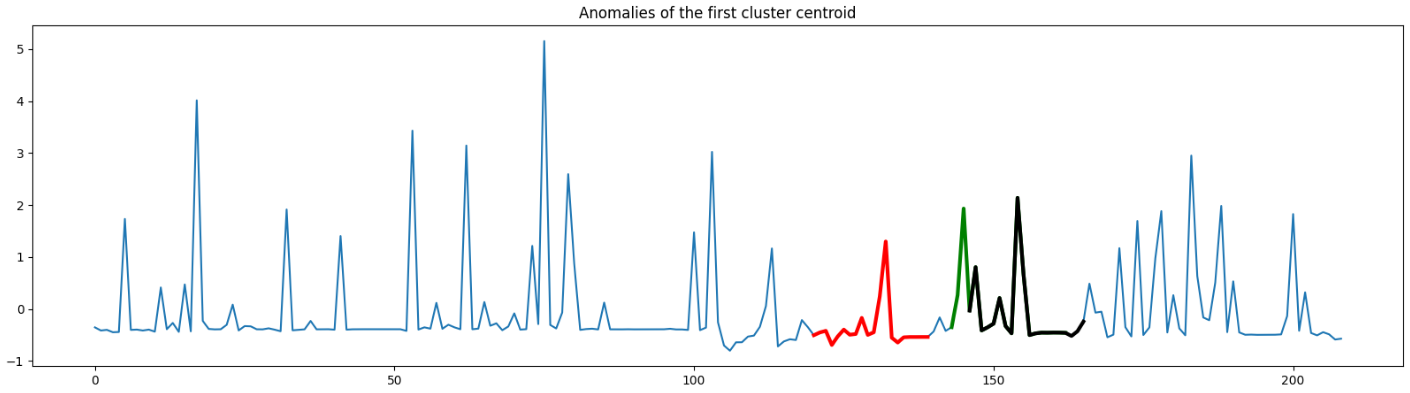
\includegraphics[width=.99\textwidth]{img/ts/Anom1.png}
      
        \label{ANOM1}
    \end{figure}
    
    \begin{figure}
        \centering
        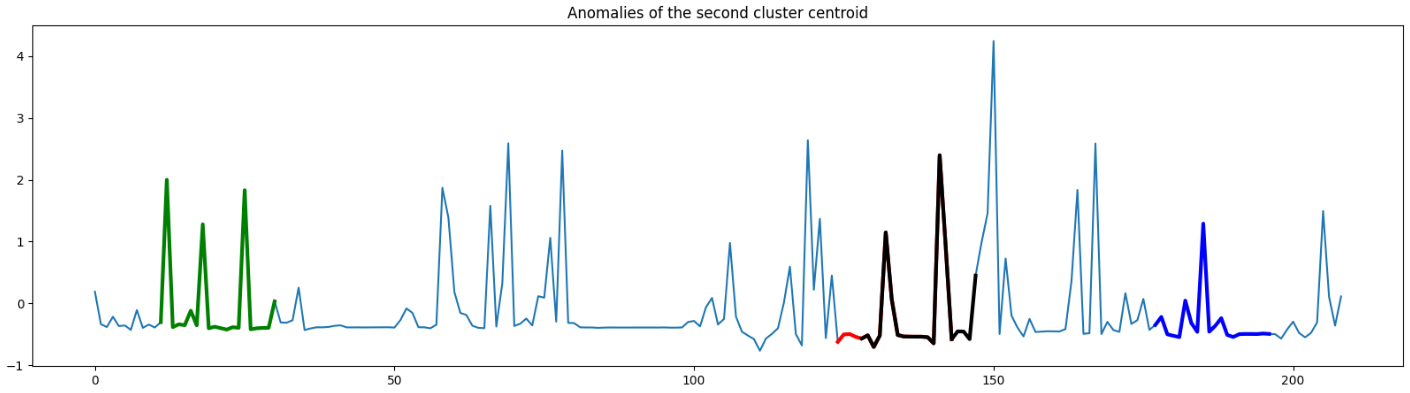
\includegraphics[width=.99\textwidth]{img/ts/Anom2.png}
      
        \label{ANOM2}
    \end{figure}
    
    
        
\end{frame}


%%%%%%%%%%%%%%%%%%%%%%%%%%%%%%%%%%%%%%%%%%%%%%%%%%%%%%%%%%%%%%%%%%%%%%%%%%


\begin{frame}{New Score}


    \begin{exampleblock}{\textsc{New\_Score = }}
        \begin{flalign*}
            n\_incidents\_week + n\_participants\_week
        \end{flalign*}
        \begin{flalign*}
            &n\_incidents\_week = \text{number of incidents in a specific week} \\
            &n\_participants\_week = \text{number of participants of all the incidents }\\
            &\text{in a specific week }
        \end{flalign*}
    \end{exampleblock}
    
\end{frame}
    

%%%%%%%%%%%%%%%%%%%%%%%%%%%%%%%%%%%%%%%%%%%%%%%%%%%%%%%%%%%%%%%%%%%%%%%%%%

\begin{frame}{ROC and Precision curve}
    \begin{figure}
        \centering
        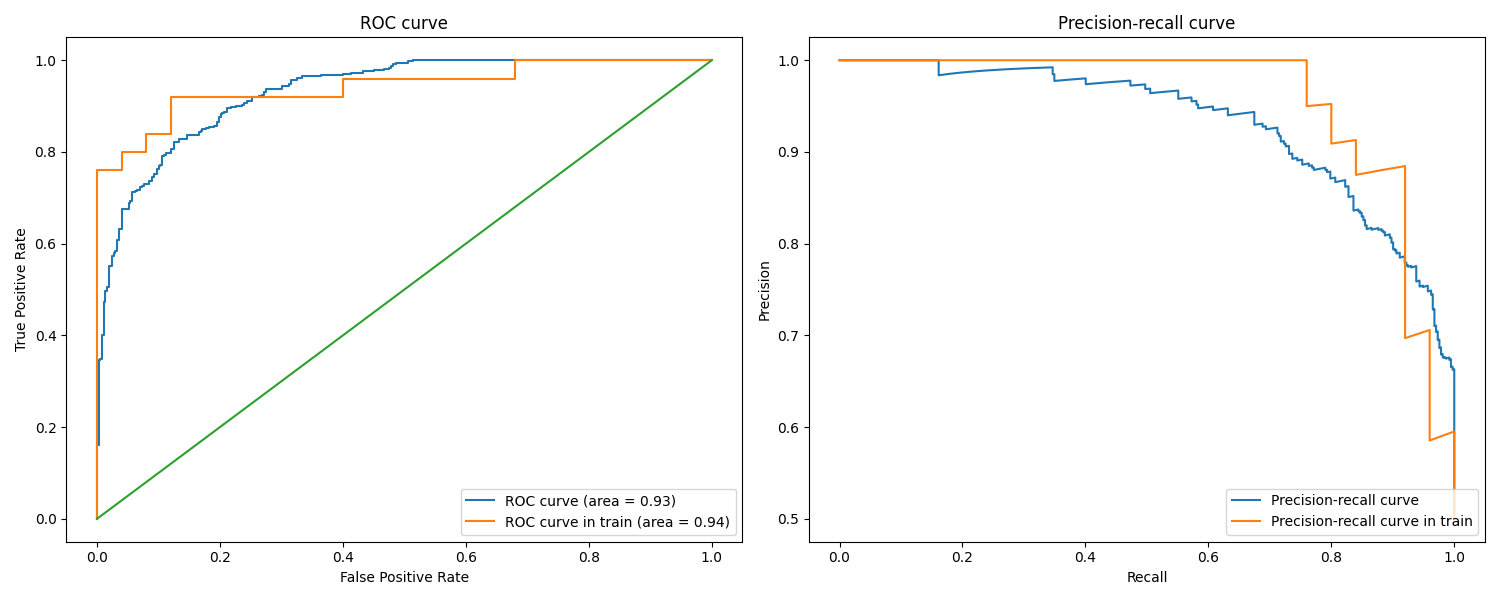
\includegraphics[width=.99\textwidth]{img/ts/roc_pr.png}
    
        \caption{ROC curve and Precision curve of the classifier}
        \label{ROC}
    \end{figure}
\end{frame}


%%%%%%%%%%%%%%%%%%%%%%%%%%%%%%%%%%%%%%%%%%%%%%%%%%%%%%%%%%%%%%%%%%%%%%%%%%

\begin{frame}{Confusion Matrix}
    \begin{figure}
        \centering
        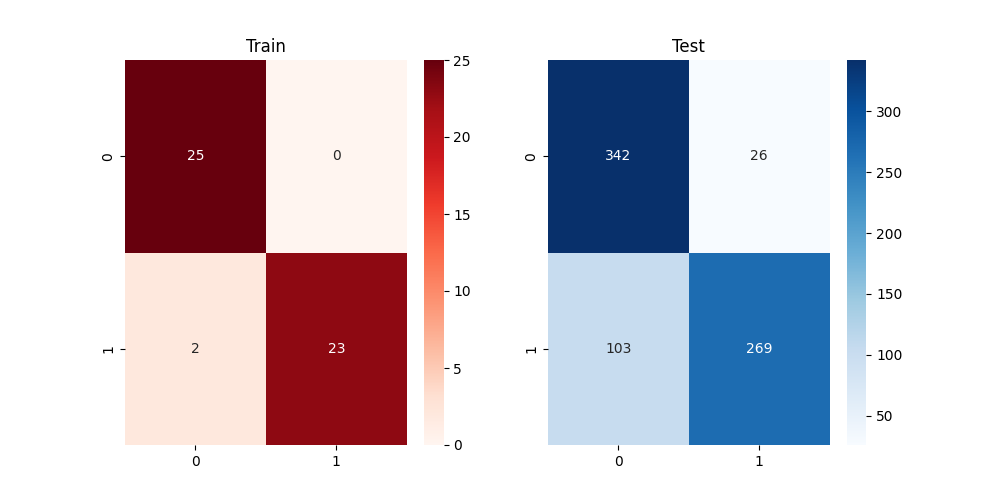
\includegraphics[width=.99\textwidth]{img/ts/confusion_matrix.png}
    
        \caption{Train and Test set Confusion Matrices}
        \label{MTX}
    \end{figure}
\end{frame}
    
    